\section{Технологический раздел}

\subsection{Выбор средств разработки}

В данном разделе рассматриваются такие инструменты разработки, как язык программирования, среда разработки и используемые библиотеки.

В первом подразделе будет описан язык программирования, который был выбран для реализации программного продукта, а также были описаны необходимые библиотеки для реализации поставленной задачи. Как для языка, так и для используемых библиотек были описаны преимущества их использования и обоснованность выбора именно данного языка и библиотек.

\subsubsection{Язык программирования и используемые библиотеки}

В качестве языка программирования для разработки программного продукта было принято решение использовать язык Python v3.9.2. Преимуществом данного языка является большое разнообразие представленных библиотек и фреймворков, а также обладает большой гибкостью и удобством использования.

При разработке программного обеспечения использовались следующие библиотеки и фреймворки:

\begin{itemize}
	\item NumPy --- библиотека, поддерживающая работу с большими
	многомерными массивами и матрицами, а также предоставляющая
	набор математических функций для работы с этими данными \cite{NumPy};
	\item Pandas --- библиотека, предоставляющая удобные структуры и операции для работы с табличными даннами \cite{Pandas};
	\item Scikit-learn --- данная библиотека включает в себя различные алгоритмы машинного обучения и подготовку данных для последующей;
	классификации, поддерживает взаимодействие с NumPy и Pandas \cite{Scikit-learn};
	\item SciPy --- библиотека для математического и числового анализа, такого как вычисление косинусной близости \cite{SciPy};
	\item NLTK --- библиотека для работы с текстовыми данными, предоставляющая возможности обработки и лемматизации текста \cite{NLTK}; 
	\item Django --- бесплатный высокоуровневый веб-фреймворк \cite{Django}.
\end{itemize}

\subsubsection{Среда разработки}

В качестве среды разработки модуля рекомендательной системой было решено использовать IDE Jupyter Notebook так как он позволяет выполнять код по ячейкам, что очень удобно для разработки модулей, использующих методы машинного обучения. Для разработки графического интерфейса рекомендательной системы была использована IDE PyCharm, которая предоставляется студентам бесплатно по лицензии, а также предоставляет возможности создания виртуальной среды разработки для быстрой установки новых библиотек и модулей.

\subsection{Структура разработанного ПО}

Структура разработанного ПО в виде UML диаграммы представлена на рисунке \ref{uml}.

\begin{figure}[H]
	\centering
	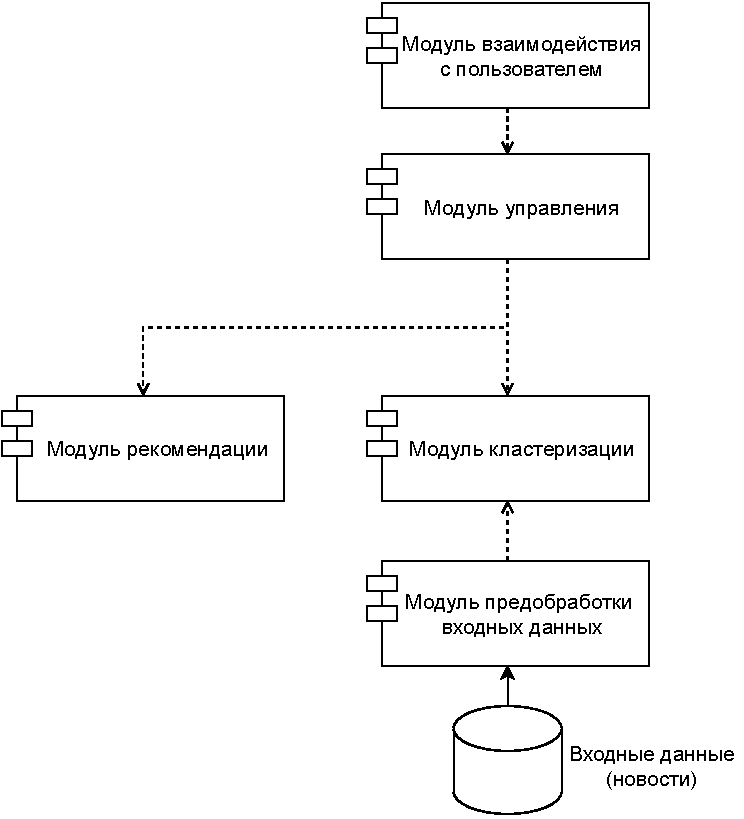
\includegraphics[width=\textwidth]{img/UML.pdf}
	\caption{UML диаграмма разработанного ПО}
	\label{uml}
\end{figure}  

Каждый из модулей, изображенный на диаграмме, содержит сгруппированные по функциональному значению соответствующие классы. Модуль взаимодействия с пользователем отвечает за пользовательский интерфейс. Модуль управления объединяет модуль рекомендации и модуль кластеризации и координирует их работу.

\subsection{Пользовательский интерфейс}

Интерфейс представляет из себя две веб-страницы с новостями. Веб-страница реализована на HTML с использованием CSS стилей. В качестве веб-фреймворка использовался Django.

Пример работы программы в случае если пользователь находится на главной странице и в случае если он находится на странице с новостью, представлены на рисунках \ref{prog_1}, \ref{prog_2}.

\begin{figure}[H]
	\centering
	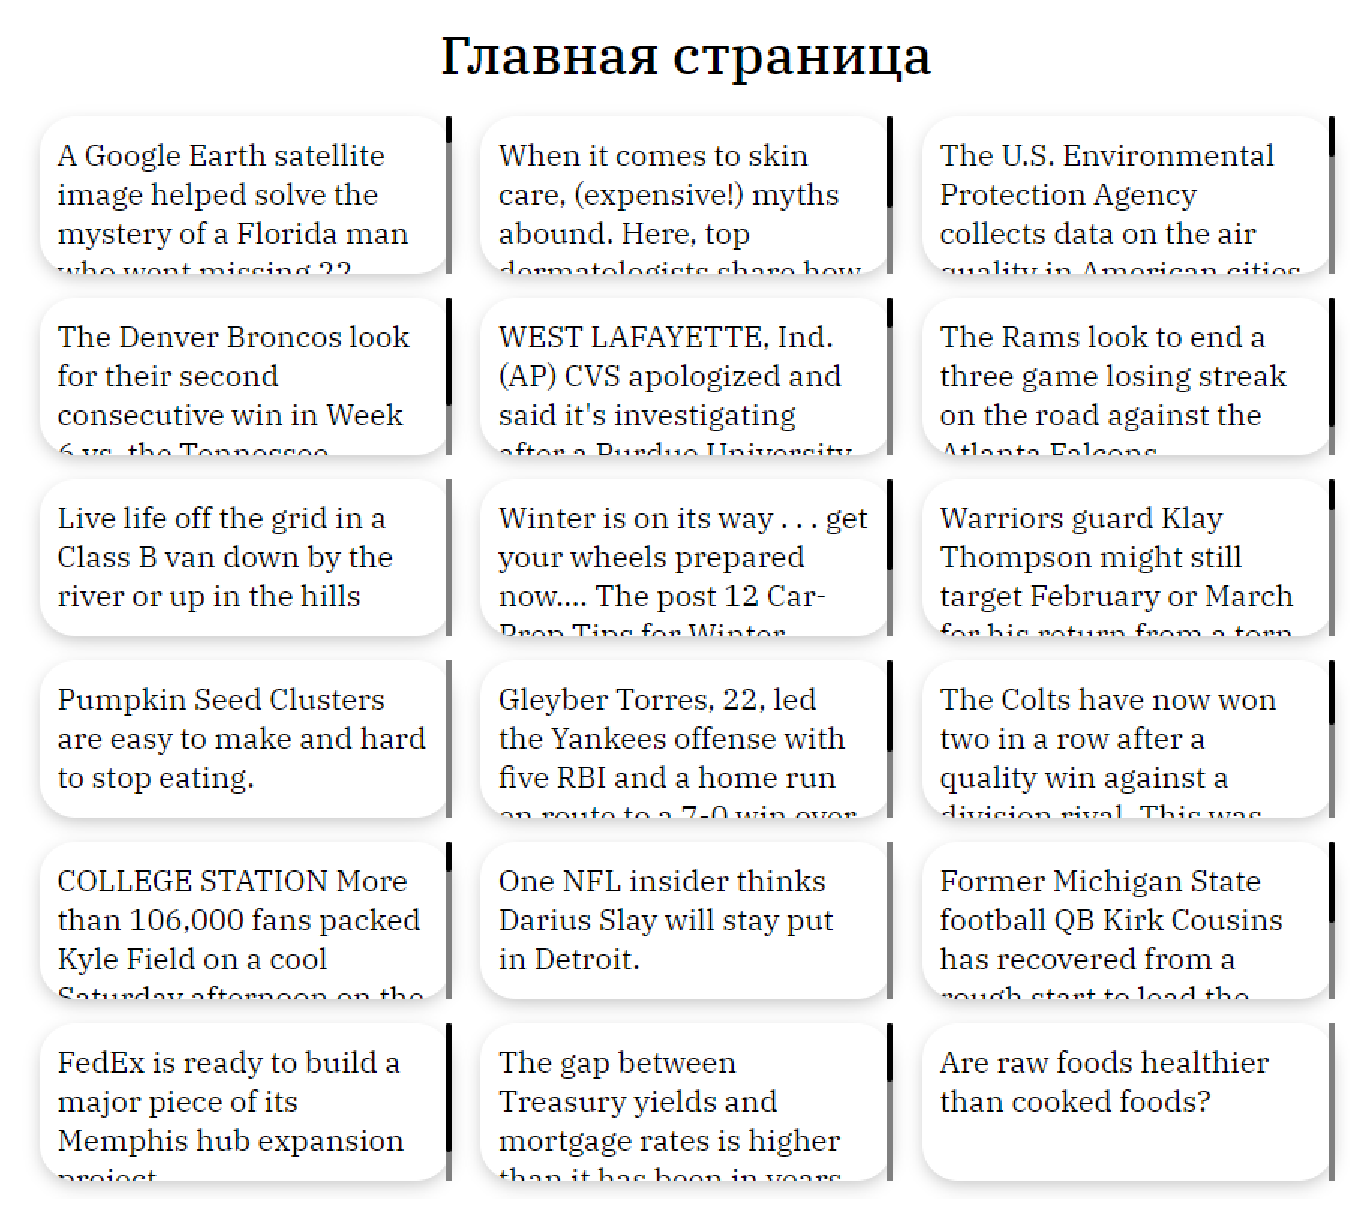
\includegraphics[width=\textwidth]{img/prog_1.pdf}
	\caption{Пример работы программы главной страницы новостного сайта}
	\label{prog_1}
\end{figure}  

\begin{figure}[H]
	\centering
	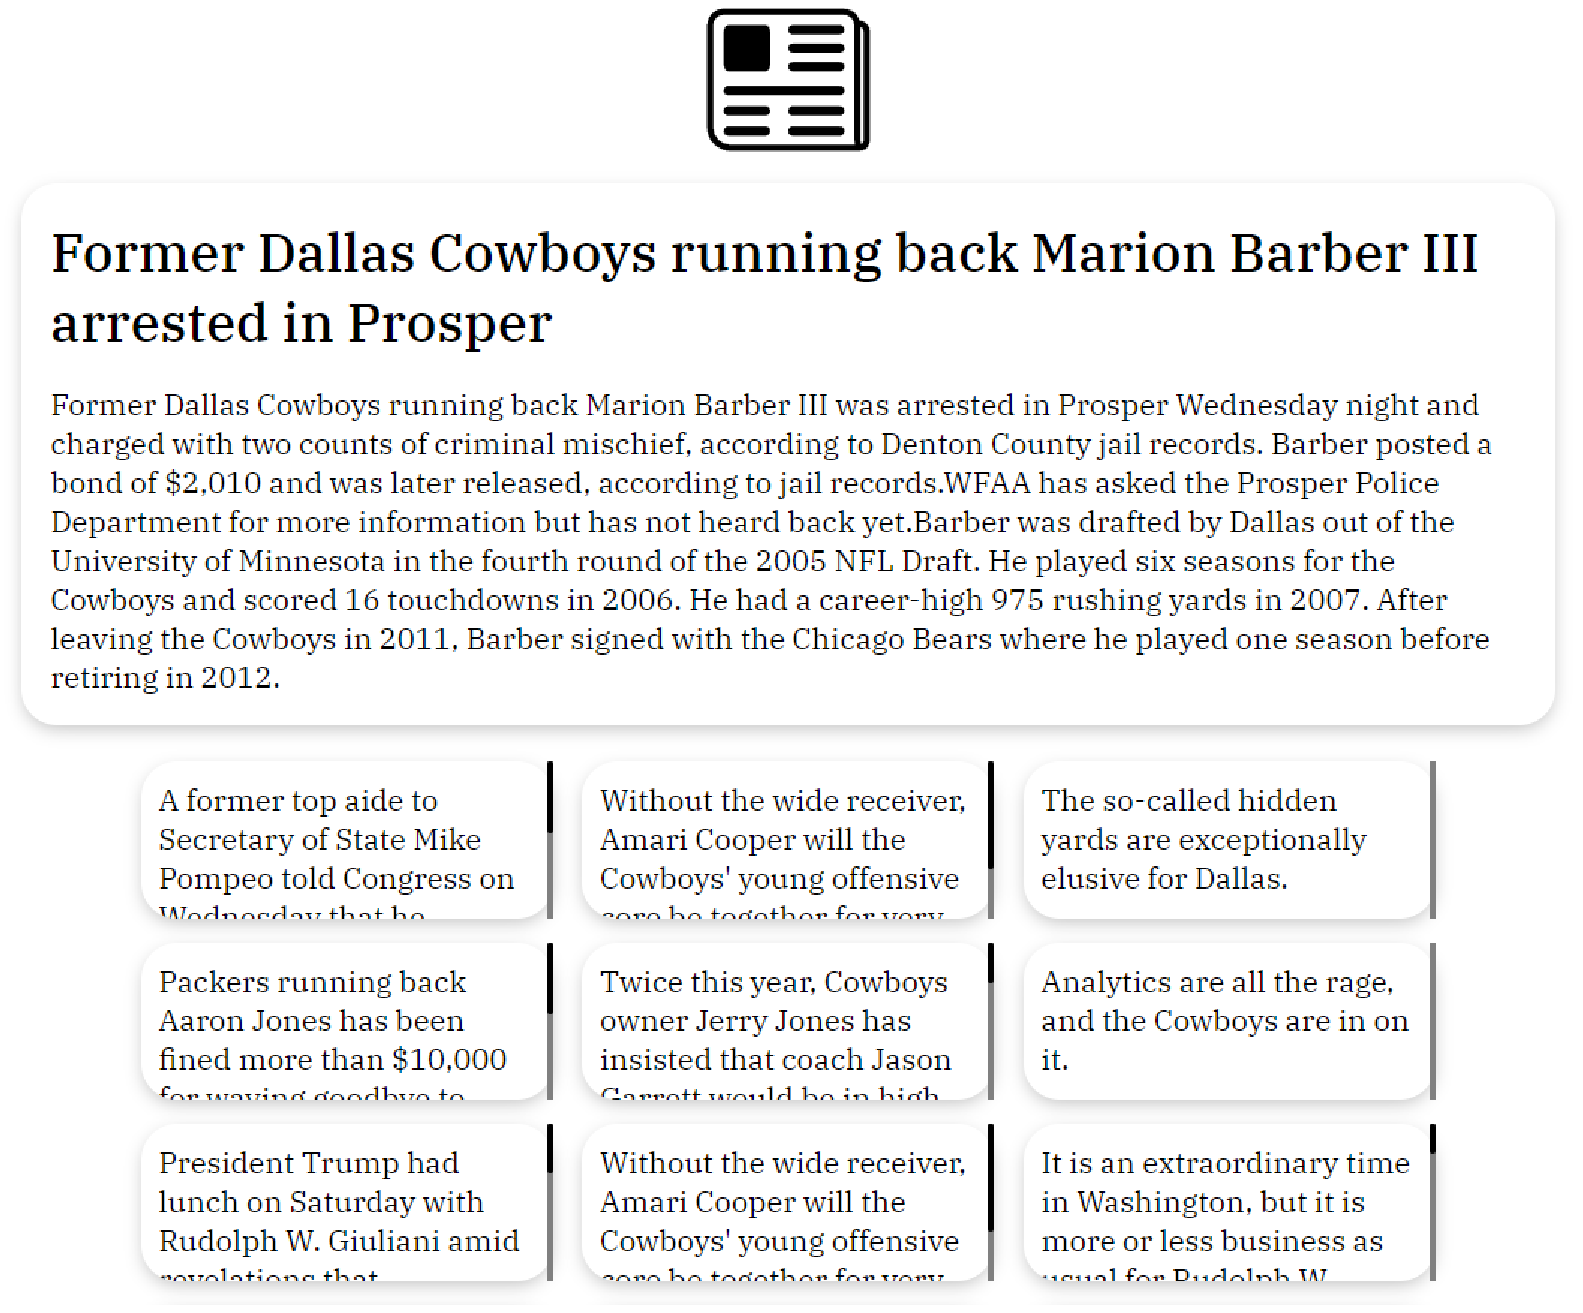
\includegraphics[width=\textwidth]{img/prog_2.pdf}
	\caption{Пример работы программы страницы с новостью}
	\label{prog_2}
\end{figure}  

Далее будет приведен пример работы программы в случае если пользователь добавляет новость, к примеру про бои UFC и страница с рекомендациями на основе, добавленной новости. На рисунке \ref{prog_3} страница добавления новости, а на рисунке \ref{prog_4} страница добавленной новости и рекомендаций на ее основе.

\begin{figure}[H]
	\centering
	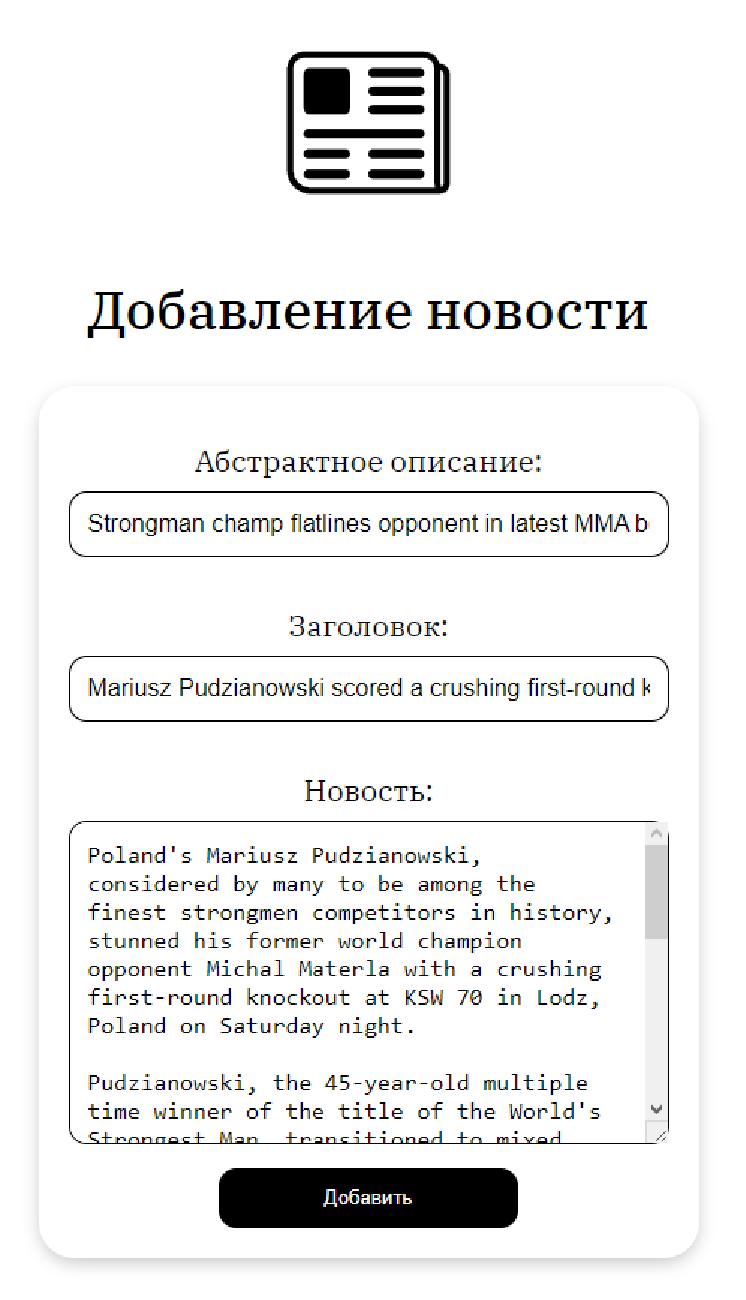
\includegraphics[scale=1]{img/prog_3.pdf}
	\caption{Пример работы программы страницы добавления новости}
	\label{prog_3}
\end{figure}  

\begin{figure}[H]
	\centering
	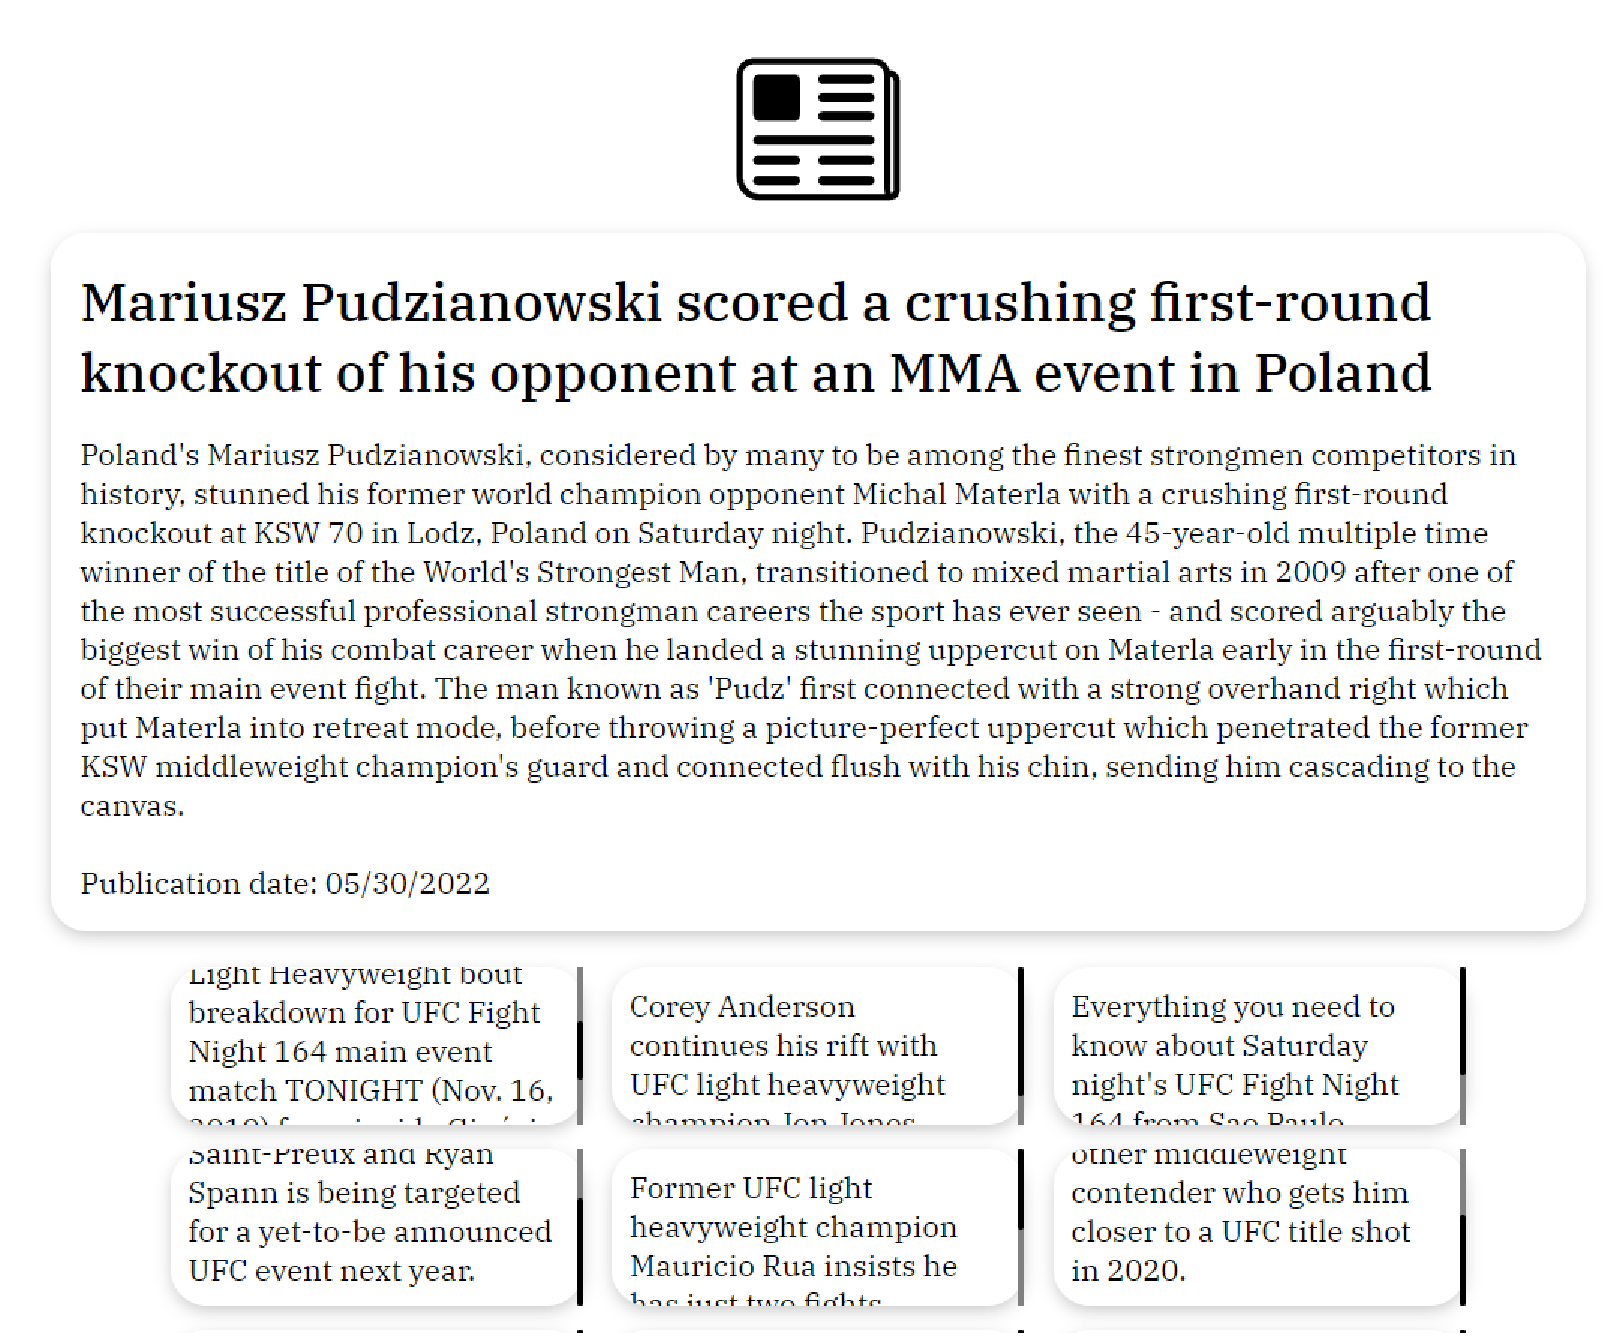
\includegraphics[width=\textwidth]{img/prog_4.pdf}
	\caption{Страница с добавленной новостью и рекомендациями к ней}
	\label{prog_4}
\end{figure}  

Как можно заметить, все рекомендации так или иначе связаны с боями UFC, что говорит о хорошем качестве предсказания новостей к рекомендации.

\subsection{Выводы из технологического раздела}

В данном разделе были описаны средства реализации, которые были использованы для разработки ПО, после чего были приведены выбранные инструменты, обоснованы причины их использования и преимущества.

Была описана структура разработанного программного обеспечения и приведено описание каждого из модулей, приведенного на UML диаграмме. Также был приведен пользовательский интерфейс программы и продемонстрирован пример работы программы в случае просмотра и добавления новости.

\pagebreak